% Partial recreation. All uncertain indices/primes are explicitly bracketed.
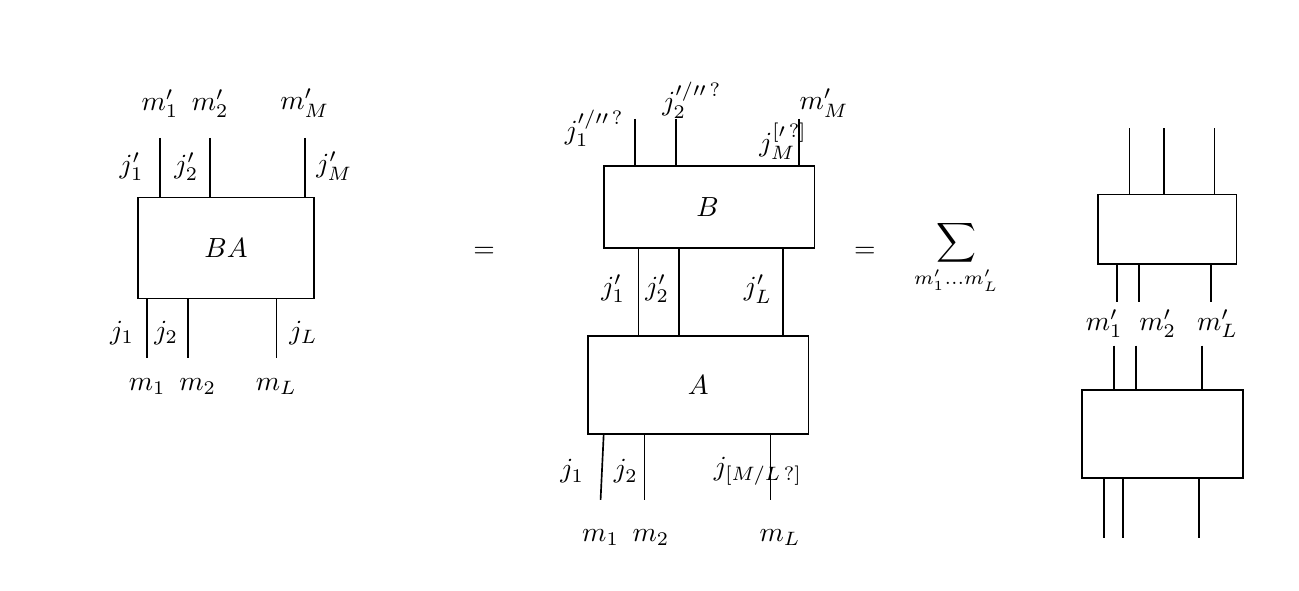
\begin{tikzpicture}[x=0.008cm,y=-0.008cm,line width=0.6pt]
\path[use as bounding box] (0,0) rectangle (1975,850);
\draw (175,270) rectangle (455,430);
\node at (315,350) {$BA$};
\foreach \x in {210,290,440}{\draw (\x,175)--(\x,270);}
\foreach \x in {190,255,395}{\draw (\x,430)--(\x,525);}
\node at (210,120) {$m'_1$};\node at (290,120) {$m'_2$};\node at (440,120) {$m'_M$};
\node at (165,220) {$j'_1$};\node at (252,220) {$j'_2$};\node at (487,220) {$j'_M$};
\node at (150,485) {$j_1$};\node at (220,485) {$j_2$};\node at (438,485) {$j_L$};
\node at (190,570) {$m_1$};\node at (270,570) {$m_2$};\node at (395,570) {$m_L$};
\node at (725,357) {$=$};
\draw (915,220) rectangle (1250,350);\node at (1080,285) {$B$};
\draw (890,490) rectangle (1240,645);\node at (1065,567) {$A$};
\foreach \x in {965,1030,1225}{\draw (\x,145)--(\x,220);}
\draw (970,350)--(970,490);\draw (1035,350)--(1035,490);\draw (1200,350)--(1200,490);
\draw (915,645)--(910,750);\draw (980,645)--(980,750);\draw (1180,645)--(1180,750);
\node at (900,160) {$j_1^{\prime/\prime\prime\,?}$};
\node at (1055,115) {$j_2^{\prime/\prime\prime\,?}$};
\node at (1200,180) {$j_M^{[\prime\,?]}$};\node at (1265,120) {$m'_M$};
\node at (930,415) {$j'_1$};\node at (1000,415) {$j'_2$};\node at (1160,415) {$j'_L$};
\node at (865,705) {$j_1$};\node at (950,705) {$j_2$};\node at (1160,705) {$j_{[M/L\,?]}$};
\node at (910,810) {$m_1$};\node at (990,810) {$m_2$};\node at (1195,810) {$m_L$};
\node at (1330,357) {$=$};\node at (1475,365) {$\displaystyle\sum_{m'_1\ldots m'_L}$};
\draw (1700,265) rectangle (1920,375);\draw (1675,575) rectangle (1930,715);
\foreach \x in {1750,1805,1885}{\draw (\x,160)--(\x,265);}
\foreach \x in {1730,1765,1880}{\draw (\x,375)--(\x,435);}
\foreach \x in {1725,1760,1865}{\draw (\x,505)--(\x,575);}
\foreach \x in {1710,1740,1860}{\draw (\x,715)--(\x,810);}
\node at (1710,470) {$m'_1$};\node at (1795,470) {$m'_2$};\node at (1890,470) {$m'_L$};
\end{tikzpicture}
